\chapter{Background}
\label{chapter:background}
\section{Call and Put Options}
As stated before, call and put options enable their buyer to buy and sell the underlying stock at the maturity for the fixed strike price.
In the case of a call option, if at the maturity the price of its underlying asset is greater than the strike, an investor can buy it for the latter and immediately sell it for its higher market price. Thus, the payoff of the option would be the difference of these two values. On the other hand, if the price of the asset decreases past the strike at the maturity, the investor should let the option expire, since the asset is available for a price in the market price lower than the higher strike. In this case, the payoff of the option would be zero.
The same reasoning can be made for put type options.
The payoff function of these two types of options can then simply be deduced as
\begin{equation}\label{callput}
\begin{split}
&\text{Payoff}_\text{call}=\max\left(S(T)-K,0\right);\\
&\text{Payoff}_\text{put}=\max\left(K-S(T),0\right),
\end{split}
\end{equation}
\noindent where $K$ is the strike price and $S(T)$ is the asset price, $S(t)$, at the maturity, $T$. These functions are represented in \autoref{fig:Payoff}.

\begin{figure}[!htb]
    \centering
      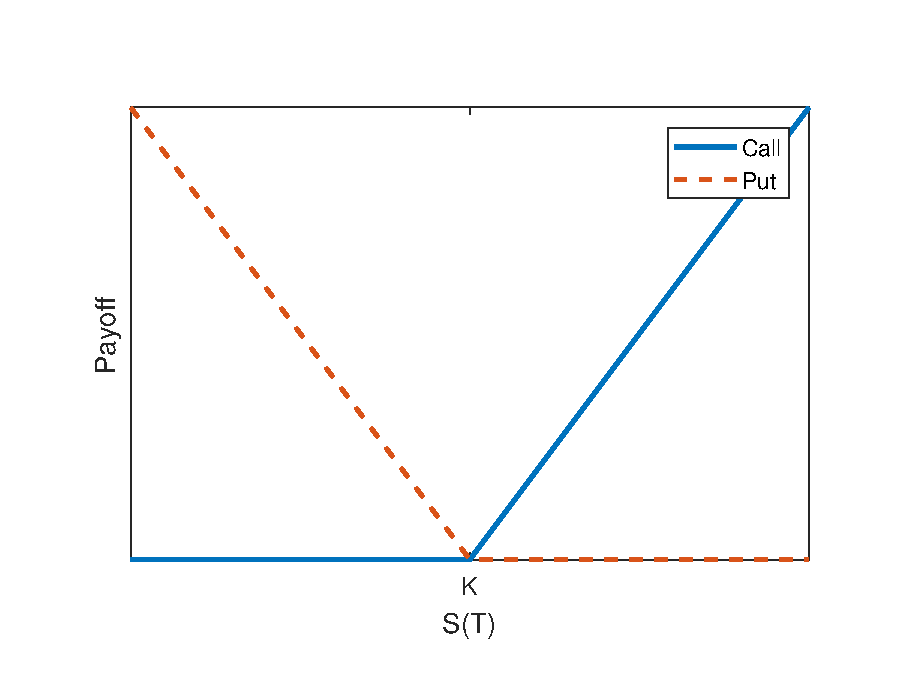
\includegraphics[width=.5\columnwidth]{Payoff.eps}
      \caption[Payoff functions of call and put options]{Payoff functions of \emph{call} and \emph{put options}.}\label{fig:Payoff}
    \end{figure}
    
\section{Black-Scholes-Merton Formulae}
\label{section:Black-Scholes-Merton Formulae}
Due to their high importance, options have been studied in great detail in the past.
Probably the most important result in this field came from Fischer Black, Myron Scholes and Robert Merton, who developed a mathematical model to price options~~\cite{Scholes} - the famous Black-Scholes-Merton model - still in use in present days~~\cite{Wilmott}. The last two actually earned the 1997 Nobel prize in Economics for this development.

This model states that the price of an European call or put option, whose underlying asset is a stock, follows the partial differential equation (PDE)

\begin{equation}\label{BS2}
\pdv{V}{t}+\frac{1}{2}\sigma^2S^2\pdv{^2V}{S^2}+rS\pdv{V}{S}-rV=0,
\end{equation}

\noindent where $V$ is the price of the option, $S$ is the price of the underlying stock, $r$ is the risk-free interest rate and $\sigma$ is the stock price volatility.

The risk-free interest rate, $r$, is the interest an investor would receive from a risk-free investment. An investor should never invest in risky products whose expected return is lower than this interest, since there's the alternative of investing without risk. In general, this rate changes slightly with time, but Black \textit{et al.} assumed, in their original model, that it remains constant throghout the option duration. Some later developments dealt with this shortcoming, but because option prices do not significantly depend on this value~~\cite{Wilmott}, in the remainder of this thesis we shall assume it is constant and known.

Finally, the volatility, $\sigma$, is a measure of uncertainty and will be studied in more detail in section \ref{section:volatility}.

One important assumption of this model is that stock prices follow a Geometric Brownian Motion (GBM), defined as
\begin{equation}\label{GBM}
dS(t)=rS(t)dt+\sigma S(t)dW(t),
\end{equation}
\noindent with $\{W(t),\ t>0\}$ defining a one-dimensional Brownian motion.


Pricing options is fairly straightforward - we simply need to solve the PDE in eq. \eqref{BS2} in a similar fashion to the initial value problem for the diffusion equation~~\cite{Dilao}.
The results published in the original article by Black \textit{et al.} state that, at time $t$, call and put options can be valued as
\begin{equation}\label{callputBS}
\begin{split}
&C(S(t),t)=N(d_1)S(t)-N(d_2)Ke^{-r(T-t)};\\
&P(S(t),t)=-N(-d_1)S(t)+N(-d_2)Ke^{-r(T-t)},
\end{split}
\end{equation}
\noindent where $N(\cdot)$ is the cumulative distribution function of the standard normal distribution, $T$ is the maturity time, and $d_1$, $d_2$ are given by
\begin{equation}\label{d1d2}
\begin{split}
&d_1=\frac{1}{\sigma\sqrt{T-t}}\left[\ln\left(\frac{S_t}{K}\right)+\left(r+\frac{\sigma^2}{2}\right)(T - t)\right];\\
&d_2=d_1-\sigma\sqrt{T-t}.\\
\end{split}
\end{equation}



From eq. \eqref{callputBS} we can derive a relationship between $C(S,t)$ and $P(S,t)$, known as the \emph{put-call parity}
\begin{equation}
C(S(t),t)=S(t)-Ke^{-r(T-t)}+P(S(t),t).
\end{equation}
\noindent Because of this duality, we can always obtain the prices of put options from call options with the same underlying asset, maturity and strike. For this reason, unless otherwise stated, all options will be assumed calls in the following sections.


\section{Volatility}
\label{section:volatility}
Volatility is a measure of the uncertainty of future stock prices changes. In other words, a high volatility will lead to great future fluctuations in the stock price, whereas a stock with low volatility is more stable.

Of all the parameters in the Black-Scholes formula, \eqref{BS2}, volatility is the only one we can't easily observe from market data.
Furthermore, unlike the interest rate, volatility has a great impact on the behavior of stock prices and consequently on the price of options.
These two factors make volatility one of the most studied subjects in option pricing.



It should be noted that there are several types of volatility, depending on what is being measured. Some of these types will be approached in the next subsections.

\subsection{Implied Volatility}
\label{section:impliedvolatility}
The \emph{implied volatility} can be described as the value of stock price volatility that, when input into the Black-Scholes pricer in eq. \eqref{callputBS}, outputs a value equal to the market price of a given option.
In other words, it would be the stock volatility that the seller/buyer of the option assumed when pricing it (given that the Black-Scholes model was used).

Because eq. \eqref{callputBS} is not invertible, we need to use some numerical method (e.g Newton's method) to find the solution to the equation
\begin{equation}
C(\sigma_{imp},S(t),t)-\overline{C}=0,
\end{equation}
\noindent where $C(\sigma_{imp},\cdot)$ corresponds to the solution of eq. \eqref{callputBS} using the implied volatility $\sigma_{imp}$ and $\overline{C}$ is the price of the option observed at the market.

We can obtain the implied volatility of an option from its price or the price from its implied volatility, because eq. \eqref{callputBS} is monotonic in the volatility. This duality is so fundamental that exchanges sometimes sell their options providing only the implied volatility instead of the price~\citep{Wilmott}.

One interesting property of implied volatility is that, in the real-world, it varies with the strike price and maturity. In principle, if investors really used the Black-Scholes model to price their options, two options with the same underlying asset should have the same implied volatility, despite their strike prices or maturities.
However, when observing market data, this is not the case. The observed implied volatilities form two possible shapes in a scatter plot, known as \emph{smile} and \emph{skew}.
An implied volatility smile shows greater $\sigma_{imp}$ for options with strikes different from the current stock price and the minimum where the strike equals the stock price. A skew, on the other hand, only shows greater $\sigma_{imp}$ in one of the directions (i.e. for strikes either higher or lower than the current stock price). You can observe both these phenomena in \autoref{fig:smileskew}.
We can therefore conclude that options with strikes different from the current stock price are overpriced.
The reason behind this odd market behavior is the simple demand-supply rule~\citep{Wilmott}. On the one hand, some investors are risk-averse and want to hedge their losses in case of a market crash (as explained in subsection \ref{subsection:why options are important}). They don't mind paying a higher price for an option if this means they would be safe from crashes. For this reason, the prices of low strike (call) options increase which drives their implied volatility up. On the other hand, some other investors are risk-seekers and want to take advantage of possible sudden price increases, buying the stocks for lower prices. They don't mind paying higher prices for the options and this drives the prices of high strike options (and, consequently, their implied volatility) up.
    
    
\begin{figure}[!htb]
  \begin{subfigmatrix}{2}
    \subfigure[Smile]{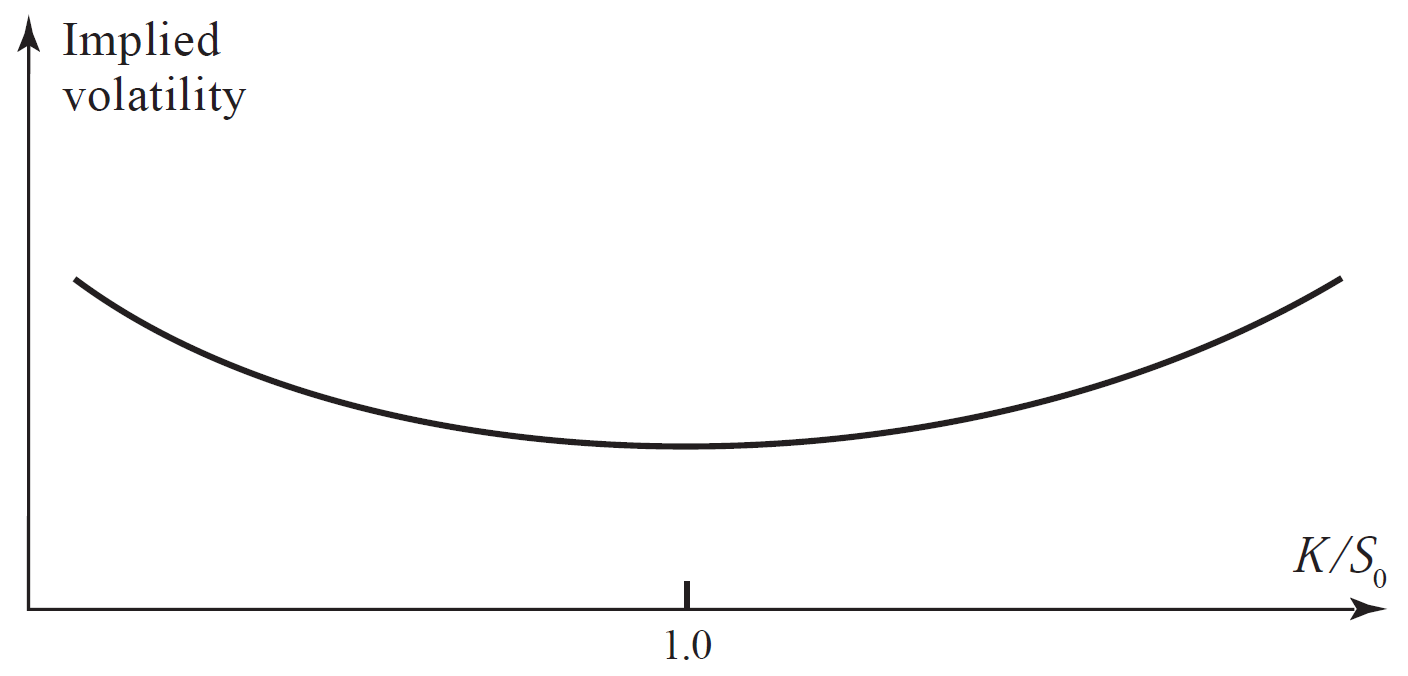
\includegraphics[height=0.20\linewidth]{Smile.png}}
    \subfigure[Skew]{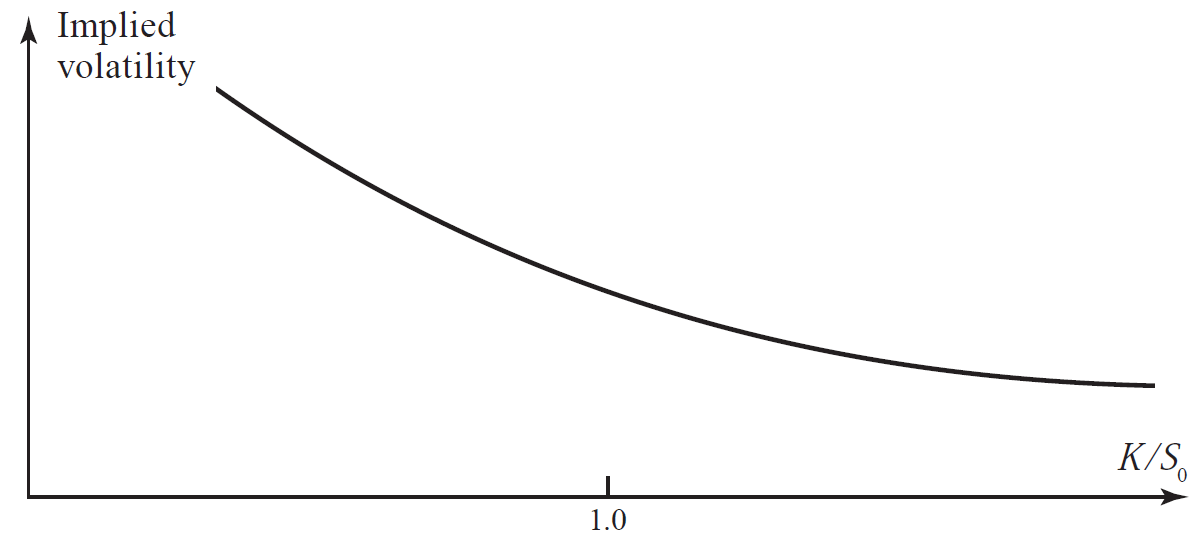
\includegraphics[height=0.20\linewidth]{Skew.png}}
  \end{subfigmatrix}
  \caption[Example of an implied volatility smile and skew.]{Example of an implied volatility smile and skew.\hl{source=Hull}}
  \label{fig:smileskew}
\end{figure}

\subsection{Local Volatility}
\label{subsection:localvolatility}
In their original work, Black \textit{et al.} assumed that volatility is constant throughout the whole contract. From market data, it can be clearly seen that this is not the case. There may be times where new information reaches the market and trading increases, driving volatility up. The opposite is also true.

The model in eq. \eqref{callputBS} is clearly not enough to truly grasp real-world trading. We should have a model where volatility is dynamic, measuring the amount of randomness in the stock price at any given time.
The geometric Brownian motion from eq. \ref{GBM} would thus become
\begin{equation*}
dS(t)=rS(t)dt+\sigma(t)S(t)dW(t),
\end{equation*}
\noindent where $\sigma(t)$ is now some function of time.


However, as we saw in subsection \ref{section:impliedvolatility} for implied volatility, the market's view of volatility also varies with the strike price. A simple dynamic volatility model is thus unsufficient. The local volatility should then be a function of both time and strike price. We are left with a new GBM, given by
\begin{equation}\label{GBM2}
dS(t)=rS(t)dt+\sigma(K,t)S(t)dW(t),
\end{equation}
\noindent where $\sigma(K,t)$ depends now on $K$ and $t$.


Finding the local volatility function is not very important when pricing typical European options, because we can simply use the implied volatility in eq. \ref{GBM} and assume it remains constant.
However, for other contracts, such as American, Asian or Barrier options (among others) where the option value depends on the path the stock price takes, this function is indeed crucial.

The local volatility function is very difficult to calibrate, because we can't directly measure the local volatility of a stock from market data. 
Some models have been proposed in an attempt to achieve this goal. The most well known model is known as Dupire's formula.

\subsubsection{Dupire's Formula}
\label{subsubsection:Dupire}
One of the most famous results in the modelling of the local volatility function was obtained by Dupire~\cite{Dupire}. In his article, he derives a theoretical formula for this function, given by
\begin{equation}\label{dupire}
\sigma(K,T)=\sqrt{\frac{\displaystyle\pdv{C}{T}+rK\pdv{C}{K}}{\displaystyle\frac{1}{2}K^2\pdv{^2C}{K^2}}},
\end{equation}
\noindent where $\sigma(K,T)$ is the volatility function for stock prices $K$ at time $T$ and $C=C(K,T)$ is the price of an European call option with strike price $K$ and maturity $T$.
A brief demonstration of this formula can be found in appendix \ref{chapter:dupireformuladerivation}.


As can be seen, we need to differentiate the option prices with respect to their strikes and maturities. To achieve this, we need to gather a large number of option prices from the market, for options with different maturities and strikes, and interpolate between them to obtain an option price surface (with $K$ and $T$ as variables). We then calculate the gradients in this surface and input them into eq. \ref{dupire} to obtain the local volatility surface.

Even before implementation, four potential sources of error can be found.
First, it should be noted that markets only trade options with very specific maturities (e.g. 1, 2, 4, 6-months maturity). For this reason, our data will be very sparse with respect to maturity and the interpolation obtained may not closely resemble reality.
Furthermore, it can be seen that we are dividing by the second derivative with respect to the strike price. \hl{As we will see in the next section}, the prices of options with strikes very far from the current stock price change at an approximately constant rate with respect to the strike. The second derivative in these regions would then be very close to or actually zero. Because we are dividing by this value, our volatilities may explode for very large or very small strikes.
Then, there is the problem of noise. Because we are interpolating very sparse data, even small errors in the option market price will cause variations in the interpolation which can be very problematic if the second derivative changes, because we are dividing by it.
Finally, some problems arise from the market itself. While investors use mathematical finance in their trades, the market is still governed by the demand-supply rule. If many investors want to buy the option and few want to sell it, the option price will increase, even if it means that the option will be overpriced. It may also happen that the market is not liquid enough (i.e. very few trades or even no trades at all occur for some options) which causes the option prices to not truly follow the market's perception of future price movements.



Dupire also developed an alternative formula based on the implied volatility surface rather than the option price's.
The relation he obtained is as follows
\begin{equation}\label{dupire2}
\sigma(K,T)=\sqrt{\frac{\displaystyle\sigma_{imp}^2+2(T-t)\sigma_{imp}\pdv{\sigma_{imp}}{T}+2rK(T-t)\sigma_{imp}\pdv{\sigma_{imp}}{K}}{\displaystyle\left(1+Kd_1\sqrt{T-t}\pdv{\sigma_{imp}}{K}\right)^2+K^2(T-t)\sigma_{imp}\left(\pdv{^2\sigma_{imp}}{K^2}-d_1\left(\pdv{\sigma_{imp}}{K}\right)^2\sqrt{T-t}\right)}},
\end{equation}
\noindent where $d_1$ is given by
\begin{equation}
d_1=\frac{\log(S(t)/K)+\left(r+\frac{1}{2}\sigma_{imp}^2\right)(T-t)}{\sigma_{imp}\sqrt{T-t}},
\end{equation}
\noindent with $t$ representing the current time (usually $t=0$), $T$ being the time at which the local volatility is being measured, and $S(t)$ the stock price at time $t$. We assume that $\sigma_{imp}=\sigma_{imp}(K,T)$ is the interpolated surface of the implied volatilities evaluated at time $T$, and price $K$.
This relation might be more useful than eq. \eqref{dupire} because the implied volatility surface might be smoother than the option price's. We will compare the results from both formulas in the next chapters.


If the local volatility surface truly matched reality, it should remain constant in time, assuming the market's view of future price movements remained constant as well. However, this is not the case~\cite{Wilmott}, so we can conclude that the model doesn't completely correspond to reality and for that reason it shouldn't be used blindly.

Despite all of its shortcomings, Dupire's formula is nonetheless very much used by traders to find the local volatility surfaces of assets and price exotic options afterwards. Due to its importance, we shall implement and study this model in more detail.


\subsection{Stochastic Volatility}
\label{subsection:stochastic volatility}
As stated before, the volatility is not constant, is not observable and is not predictable, despite our attempts to model it. This seems to indicate that volatility is itself a stochastic process. Some research has been done into this hypothesis, and some models have been developed so far.

As before, we assume that the stock price follows a geometric Brownian motion
\begin{equation}
dS=rSdt+\sigma SdW_1
\end{equation}
\noindent but we further hypothesize that the volatility follows
\begin{equation}
d\sigma=p(S,\sigma,t)dt+q(S,\sigma,t)dW_2
\end{equation}
\noindent where $p(S,\sigma,t)$ and $q(S,\sigma,t)$ are some functions that depend on the model used and $W_1$ and $W_2$ are two Brownian motion processes with a correlation of $\rho$. 
\hl{This correlation can be explained by the relationship between prices and volatilities.} As an example, we can consider a stock that costs \textdollar100 and changes by \textdollar0.10 daily. We can estimate, even without calculations, that it is very stable and thus has a low volatility.
On the other hand if another stock costs \textdollar1 and changes by \textdollar0.10 in a day, we can see that it is extremely volatile even though it changed by the same amount as the first. With this example, we can see that the volatility has some correlation with the stock price.

Choosing the right $p(S,\sigma,t)$ and $q(S,\sigma,t)$ is very important in the evolution of the volatility and each stochastic volatility model will depend on the choice these functions. Furthermore, each model will have parameters that we have to calibrate using past values of the stock price. In the next subsections, we will present two of the most used models.



\subsubsection{Heston Model}
One of the most popular stochastic volatility models is known as \emph{Heston model}. It was developed in 1993 by Steven Heston~\cite{Heston} and it states that our system satisfies the relations
\begin{equation}
dS=\mu Sdt+\sqrt{\nu}SdW_1,
\end{equation}
\begin{equation}
d\nu=\kappa(\overline{\nu}-\nu)dt+\xi\sqrt{\nu}dW_2,
\end{equation}
\noindent with $\nu$ corresponding to the variance (i.e. $\nu=\sigma^2$) and where $W_1$ and $W_2$ have a correlation of $\rho$. Note that our stock price is now governed by a drift parameter $\mu$, unlike the usual risk-free measure drift of $r$, as seen in eq. \eqref{GBM}. \hl{A transformation into the risk-free measure, using Gisarnov's theorem, is possible but the original model used the drift parameter $\mu$.}
The parameters $\kappa$, $\overline{\nu}$ and $\xi$ are, respectively, the mean-reversion rate (i.e. how fast the volatility converges to its mean value), the long-term variance (i.e. the mean value of variance) and the volatility of volatility (i.e. how erratic is the volatility).

Calibrating the parameters  $\rho$, $\kappa$, $\overline{\nu}$ and $\xi$ is absolutely critical. A model with badly calibrated parameters would output wrong predictions, rendering it completely useless.
This calibration requires a fair amount of past market data and is by far the most complex and computationally demanding section of this model. We will deal with it in the next section.


\subsubsection{SABR Model}
One other very famous model of stochastic volatility was developed by Hagan \textit{et al.}~\cite{Hagan} and is known as \emph{SABR}. It stands for "\emph{stochastic-}$\alpha\beta\rho$" and in this model it is assumed that the option prices and volatilities follow
\begin{equation}\label{dF}
dF=\sigma F^\beta dW_1,
\end{equation}
\begin{equation}
d\sigma=\nu\sigma dW_2,
\end{equation}
\noindent with $\sigma(0)=\alpha$, $F(0)=f$ and where the two Brownian motion processes $W_1$ and $W_2$ have a correlation of $\rho$. It should be noted that we are now using the \hl{forward measure}, so in eq. \eqref{dF} we use $F$, the \emph{forward price}, instead of the usual spot price $S$ from eq.  \ref{GBM}. These two quantities are related by $S(t)=e^{-r(T-t)}F(t)$, so we can easily obtain one from the other.

According to Hagan \textit{et al.}, the volatility smile obtained from the local-volatility model, as developed by Dupire (eq.\eqref{dupire}), doesn't follow true market dynamics~\cite{Hagan}. They demonstrate that when the price of the asset increases or decreases, the volatility smile shifts in the opposite direction. The minimum of the volatility smile would therefore be offset and no longer correspond to the local spot price. The dynamics obtained from the local-volatility model should then be actually worse than if we assumed a constant volatility. With SABR, the authors argue that this problem is solved and the smile shifts in the correct direction.

In the original article, the authors claim that $\beta$ can be fitted from historical market data, but usually investors actually choose this value arbitrarily, depending on the type of assets traded. Typical values of $\beta$ are $\beta=1$ (stochastic lognormal model), usually used for foreign exchange options, $\beta=0$ (stochastic normal model), typical for interest rate options where forwards $f$ can be negative and $\beta=0.5$ (stochastic CIR model), also common for interest rate options.

With SABR, Hagan \textit{et al.} show that we can price new European call and put options using the typical Black-Scholes pricing equations, as in eqs. \eqref{callputBS} and \eqref{d1d2}, but replacing the implied volatility, $\sigma$, in \eqref{d1d2} with $\sigma_{SABR}$ given by
\begin{equation}\label{SABRImpvol}
\begin{split}
\sigma_{SABR}(K,f)\sim&\frac{\alpha}{\left(fK\right)^{(1-\beta)/2}\left\{1+\frac{(1-\beta)^2}{24}\log^2f/K+\frac{(1-\beta)^4}{1920}\log^4f/K\right\}}.\left(\frac{z}{x(z)}\right).\\
&\left\{1+\left(\frac{(1-\beta)^2}{24}\frac{\alpha^2}{\left(fK\right)^{1-\beta}}+\frac{1}{4}\frac{\rho\beta\nu\alpha}{\left(fK\right)^{(1-\beta)/2}}+\frac{2-3\rho^2}{24}\nu^2\right)T\right\},\\
\end{split}
\end{equation}

\noindent where $f=F(0)=S(0)e^{-rT}$, $z$ is given by
\begin{equation}
z=\frac{\nu}{\alpha}\left(fK\right)^{(1-\beta)/2}\log f/K,
\end{equation}
\noindent and $x(z)$ is
\begin{equation}
x(z)=\log\left\{\frac{\sqrt{1-2\rho z+z^2}+z-\rho}{1-\rho}\right\}.
\end{equation}

As with the Heston model, the main concern with saber is correctly calibrating the model parameters. This should take the most computational expense in the whole method.